\documentclass[a4paper]{article}
\usepackage[spanish]{babel}
\usepackage[utf8]{inputenc}
\usepackage{charter}   % tipografia
\usepackage{graphicx}
\usepackage{algorithmic}
\usepackage{amsmath}
%\usepackage{algorithm}
%\usepackage[noend]{algpseudocode}

\usepackage[bookmarks = true, colorlinks=true, linkcolor = black, citecolor = black, menucolor = black, urlcolor = blue]{hyperref} 


%\usepackage{makeidx}
\usepackage{paralist} %itemize inline
\usepackage[ruled,vlined]{algorithm2e}
%\usepackage{float}
%\usepackage{amsmath, amsthm, amssymb}
%\usepackage{amsfonts}
%\usepackage{sectsty}
%\usepackage{charter}
%\usepackage{wrapfig}
%\usepackage{listings}
%\lstset{language=C}


\usepackage{color} % para snipets de codigo coloreados
\usepackage{fancybox}  % para el sbox de los snipets de codigo

\definecolor{litegrey}{gray}{0.94}

% \newenvironment{sidebar}{%
% 	\begin{Sbox}\begin{minipage}{.85\textwidth}}%
% 	{\end{minipage}\end{Sbox}%
% 		\begin{center}\setlength{\fboxsep}{6pt}%
% 		\shadowbox{\TheSbox}\end{center}}
% \newenvironment{warning}{%
% 	\begin{Sbox}\begin{minipage}{.85\textwidth}\sffamily\lite\small\RaggedRight}%
% 	{\end{minipage}\end{Sbox}%
% 		\begin{center}\setlength{\fboxsep}{6pt}%
% 		\colorbox{litegrey}{\TheSbox}\end{center}}

\newenvironment{codesnippet}{%
	\begin{Sbox}\begin{minipage}{\textwidth}\sffamily\small}%
	{\end{minipage}\end{Sbox}%
		\begin{center}%
		\vspace{-0.4cm}\colorbox{litegrey}{\TheSbox}\end{center}\vspace{0.3cm}}



\usepackage{fancyhdr}
\pagestyle{fancy}

%\renewcommand{\chaptermark}[1]{\markboth{#1}{}}
\renewcommand{\sectionmark}[1]{\markright{\thesection\ - #1}}

\fancyhf{}

\fancyhead[LO]{Sección \rightmark} % \thesection\ 
\fancyfoot[LO]{\small{}}
\fancyfoot[RO]{\thepage}
\renewcommand{\headrulewidth}{0.5pt}
\renewcommand{\footrulewidth}{0.5pt}
\setlength{\hoffset}{-0.8in}
\setlength{\textwidth}{16cm}
%\setlength{\hoffset}{-1.1cm}
%\setlength{\textwidth}{16cm}
\setlength{\headsep}{0.5cm}
\setlength{\textheight}{25cm}
\setlength{\voffset}{-0.7in}
\setlength{\headwidth}{\textwidth}
\setlength{\headheight}{13.1pt}

\renewcommand{\baselinestretch}{1.1}  % line spacing


\usepackage{underscore}
\usepackage{caratula}
\usepackage{hyperref}

\begin{document}

\thispagestyle{empty}
\materia{Algoritmos y Estructuras de Datos III}
\submateria{Segundo Cuatrimestre de 2015}
\titulo{Trabajo Práctico I}
%\subtitulo{subtitulo del trabajo}
\integrante{Bouzón, María Belén}{128/13}{belenbouzon@hotmail.com}
\integrante{Jiménez, Paula}{655/10}{puly05@gmail.com}
\integrante{Montepagano, Pablo}{205/12}{pablo@montepagano.com.ar}
\integrante{Rey, Maximiliano}{037/13}{rey.maximiliano@gmail.com}


\maketitle
\newpage

\thispagestyle{empty}
\vfill
\begin{abstract}

\end{abstract}

\thispagestyle{empty}
\vspace{3cm}
\tableofcontents
\newpage

 \section{Objetivos generales}

\newpage
\section{Problema 1: Tel\'egrafo}

\subsection{Descripci\'on de la problem\'atica}

En el primer ejercicio se nos presenta un contexto en el que se pretende conectar con un cable de longitud arbitraria la mayor cantidad de estaciones férreas consecutivas pertenecientes a un ramal dado. 
Siéndonos provistas las distancias entre las sucesivas estaciones y la longitud del cable, la propuesta de este problema es hallar el valor de dicha cantidad.

Supongamos, por ejemplo, que nos fuera dado un ramal con cada estación  0<$i$ definida en el kilometro $j*2+2^(j-1)$ de manera tal que en un ramal de cinco estaciones las mismas se encontraran en los kilómetros 0, 3, 6, 10, 16. \\

Si contáramos con un cable de 5 kilómetros, la respuesta correcta debería ser "2", puesto que con dicha longitud se podrían unir a lo sumo dos estaciones (pudiendo ser las mismas la primera y la segunda, la segunda y la tercera o la tercera y la cuarta).\\

Si el mismo cable pudiera extenderse hasta los 6 km, la respuesta arrojada debería ser "3", representando a la combinación de las ciudades 1, 2 y 3 (cuya distancias suman exactamente 6km).\\

En cambio, si midiera 1 km, la respuesta debería ser "1", puesto que no puede conectarse más de una ciudad - sea cual fuere - con un cable de dicha longitud.\\

\subsection{Resoluci\'on propuesta y justificaci\'on}
Una primera aproximación a la resolución hubiese podido ser calcular, partiendo de cada ciudad, cuántas ciudades se pueden comunicar a partir de ella con el cable ofrecido. El problema de esta solución es que al ser `` ciego`` a los resultados parciales que cada iteración ofrece, potencialmente pueden llegar a realizarse los mismos cálculos en reiteradas oportunidades.
Por ejemplo, supongamos la siguiente distribución de las estaciones:

  \begin{figure}[h!]
   \begin{center}
 	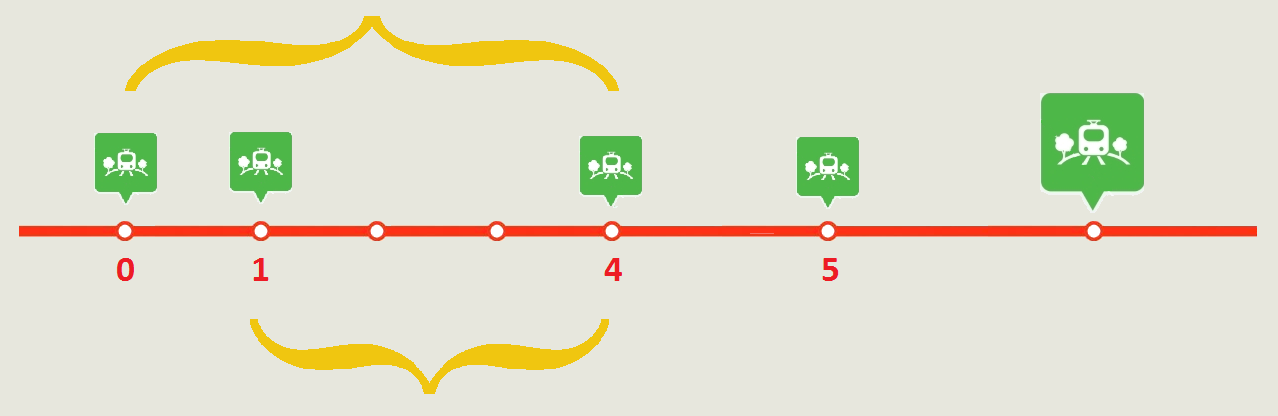
\includegraphics[scale=0.5]{imagenes/ej1/estaciones.png}
	\label{estaciones}
   \end{center}
 \end{figure}

Un algoritmo planteado a partir de esta idea, partiría de la estación Nro. 0 para concluir que se pueden conectar todas desde aquella hasta la Nro 4, para luego continuar revisando una a una las estaciones que pueden unirse partiendo de la Nro 1, cuando resulta evidente que si la distancia entre las estaciones  0 y 4 es menor o igual a la longitud del cable entonces necesariamente la distancia entre la estación siguiente (la Nro. 1) y la Nro. 4 también será menor a la longitud del cable. De no considerar esta premisa se desprende la redundancia en los cálculos que impactan en la complejidad de algoritmo. \\
 
Dicho esto, la propuesta de resolución escogida versa sobre la idea de utilizar información relevada en estaciones anteriores para aminorar la cantidad de cómputos, como se esboza en el siguiente pseudocódigo:


\begin{algorithmic} 
	
\IF{Existe alguna estación en el ramal y la longitud del cable es positiva}
	\WHILE{La estación a partir de la cuál estoy midiendo no es la última y tapoco lo es la más lejana alcanzada por dicha estación}
		\STATE Calcular la cantidad de ciudades para las cuales se sabe que alcanza el cable
		\WHILE{Alcanza el cable para unir otra estación}
			\STATE Incrementar la cantidad de estaciones que pudieron unirse
			\STATE Guardar cuál fue la estación más lejana alcanzada hasta el momento a partir de la que se mide
		\ENDWHILE
		\STATE Avanzar ciudad a partir de la cuál se mide
		\STATE Actualizar la máxima cantidad de ciudades unidas hasta el momento.
	\ENDWHILE
	\IF {Se lograron conectar dos o más ciudades}
		\STATE Devolver la maxima cantidad de estaciones que se consiguió unir.
	\ELSE
		\STATE Devolver 0
	\ENDIF
\ENDIF
\end{algorithmic}

Este procedimiento resuelve adecuadamente el problema propuesto porque calcula para cada ciudad inicial la máxima cantidad de ciudades que pueden ser recorridas y lo realiza con una cota de complejidad de O(n), como se detallará en el próximo apartado.\\

Además, como se afirma que un programa es correcto si resuelve lo pedido en una cantidad finita de pasos y sabiendo que para cualquier entrada de tama\~no N el algoritmo termina a lo sumo en $m*N$ interaciones del loop principal (con m un entero positivo) \footnote{Nótese que el bucle principal llega a su fin cuando se alcanza como ciudad base a la última estación de un ramal de N estaciones que se recorre linealmente}, podemos afirmar que nuestra solución es correcta respecto del problema presentado.\\


\newpage
\subsection{An\'alisis de la complejidad}


Sea N la cantidad total de estaciones \\

Entonces se afirma que en el peor caso cada estación va a ser estación basal en alguna instanciación del ciclo. En otras palabras, el ciclo se repetirá a lo sumo N veces.\\

Dada una instanciación del ciclo en la estación i-ésima ($i != 0$), existen dos posibilidades:
\begin{itemize}
\item	La estación $i-1$ llegó a conectar a la i-ésima y a $k$ estaciones posteriores a ella.
\item	El cable no fue lo suficientemente largo para lograrlo.
\end{itemize}

Si nos encontráramos en el segundo caso, el algoritmo partiría de la ciudad i-ésima recorriendo a lo sumo $N-i-1$ estaciones posteriores para analizar hasta cuál es la más lejana alcanzable.\\

Si el caso fuese el primero, entonces la ciudad posterior ($i$) contrastará la longitud del cable y las distancias entre kilometros para - a lo sumo - N-i-1-k estaciones (en lugar de hacerlo para N-i-1, como hubiese debido hacerlo bajo otra implementación).\\

Esto implica que para cada estación $i$, podrían llegar a realizarse a lo sumo N-i-1 comparaciones pero todas aquellas que se efectúen serán descontadas de la cantidad de cálculos que potencialmente haría la ciudad siguiente, forzando a que cada estación sea consultada acerca de su proximidad una única vez y permitiendo de esta manera que la ejecución del algoritmo se complete en tiempo lineal respecto del tamaño del input.\\ 

\newpage
\subsection{C\'odigo fuente}

A continuación se presenta la parte más relevante del código fuente, seleccionada en función de la pertinencia con la resolución del problema, dejando de lado aspectos necesarios pero secundarios, como ser el manejo de la lectura del input, la escritura del output, 
la medición de los tiempos, etc.

\begin{verbatim}

public class Main 
{
  public static void main(String[] args) throws Exception 
  {
 
	if (longitudCable != 0 && ciudades.size() > 1)
	{
	    Ramal ramal = new Ramal(ciudades);
	    int indiceCiudadMasLejanaAlcanzada    = 0;  
	    int cantMaximaCiudadesUnidas          = 1;   
	    int ciudadesUnidas;

	    while(ramal.HayCiudadesMasLejanas() &&
		 !ramal.EsLaUltimaCiudad(indiceCiudadMasLejanaAlcanzada)) 
	    {
	        if (indiceCiudadMasLejanaAlcanzada > ramal.indiceCiudadActual)
	            ciudadesUnidas =  indiceCiudadMasLejanaAlcanzada -
					 ramal.indiceCiudadActual + 1;
	        else
	            ciudadesUnidas = 1;                 

	        while(ramal.AlcanzaParaUnirUnaCiudadMas(ciudadesUnidas, longitudCable)) 
	        {
	            ciudadesUnidas ++;
	            indiceCiudadMasLejanaAlcanzada ++;
	        }
	                                
	        ramal.AvanzarCiudadBase();
	        
	        if (ciudadesUnidas > cantMaximaCiudadesUnidas)
	            cantMaximaCiudadesUnidas = ciudadesUnidas;
	        
	    }
	      
	    res = cantMaximaCiudadesUnidas == 1? 0: cantMaximaCiudadesUnidas;

	}
	else
	{
	    res = 0;
	}
  } 
}

\end{verbatim}

\newpage
\begin{verbatim}

public class Ramal {
	
    public Ramal(){}

	public ArrayList<Ciudad> ciudades;

	public Ramal (ArrayList<Ciudad> ciudades)
	{
		this.ciudades = ciudades;
		this.indiceCiudadActual = 0;
	}
	
	public int indiceCiudadActual;
	
	public boolean AlcanzaParaUnirUnaCiudadMas(int ciudadesUnidas, int longitudDeCable) 
	{
		return !EsLaUltimaCiudad(indiceCiudadActual) &&
		!EsLaUltimaCiudad(indiceCiudadActual + ciudadesUnidas - 1) &&
		DistanciaEntreCiudades(indiceCiudadActual, indiceCiudadActual + ciudadesUnidas) 
											<= longitudDeCable; 
	}
	
	public void AvanzarCiudadBase()
	{
		if (!EsLaUltimaCiudad(indiceCiudadActual))
			indiceCiudadActual++;
	}
	
	public boolean HayCiudadesMasLejanas()
	{
		return (indiceCiudadActual < ciudades.size() - 1);
	}
	
	public int DistanciaEntreCiudades(int indiceCiudadA, int indiceCiudadB)
	{
		return this.ciudades.get(indiceCiudadB).GetKilometro() -
			 this.ciudades.get(indiceCiudadA).GetKilometro();
	}

	public boolean EsLaUltimaCiudad(int indiceCiudad) 
	{
		return indiceCiudad == this.ciudades.size() - 1;
	}
}

\end{verbatim}
\newpage
\subsection{Experimentaci\'on}

Para contrastar nuestra hipótesis acerca de la complejidad temporal (presuntamente lineal) del algoritmo propuesto, diseñamos una clase denominada ClassGenerator1 encargada de generar ramales pseudoaleatorios con una cantidad de estaciones secuencialmente creciente.\\ 
La misma clase ejecuta sobre cada instancia una cantidad paramétrica de veces \footnote{350 veces, para el presente trabajo} el algoritmo que resuelve el problema propuesto. Por cada iteración sobre una misma instancia se guardan los tiempos medidos y al finalizar todas las ejecuciones sobre cada una de las instancias, se almacena en un archivo denominado $resultados.out$ el procesamiento de los datos relevados, de manera tal que persista para cada caso el promedio de los tiempos calculados sin considerar los outliers.\\
De esta forma procuramos estandarizar en la medida de lo posible los resultados, de manera que no resulten considerablemente afectados por limitaciones del hardware y del software empleado durante el análisis. \\
 \newpage

\subsubsection{Constrastaci\'on Emp\'irica de la complejidad}

Habiendo ejecutado nuestro algoritmo para 200 casos distintos donde vale que para todo $i$, caso$_{i}$ tiene un input de tamaño 10*$i$, obtuvimos resultados que expresamos visualmente en los gráficos  ~\ref{estacionesAbs} y ~\ref{estacionesRel}.\\

Mientras que el primero muestra los tiempos absolutos conseguidos para cada entrada (luego del promediado y la eliminación de outliers), el segundo presenta las razones entre los tiempos medidos para cada instancia y el tamaño de sus correspondientes parámetros de entrada. \\

En la figura \ref{estacionesRel} puede verse cómo al dividir cada tiempo computado por el tamaño del input los resultados tienden a una constante.

  \begin{figure}[h!]
   \begin{center}
 	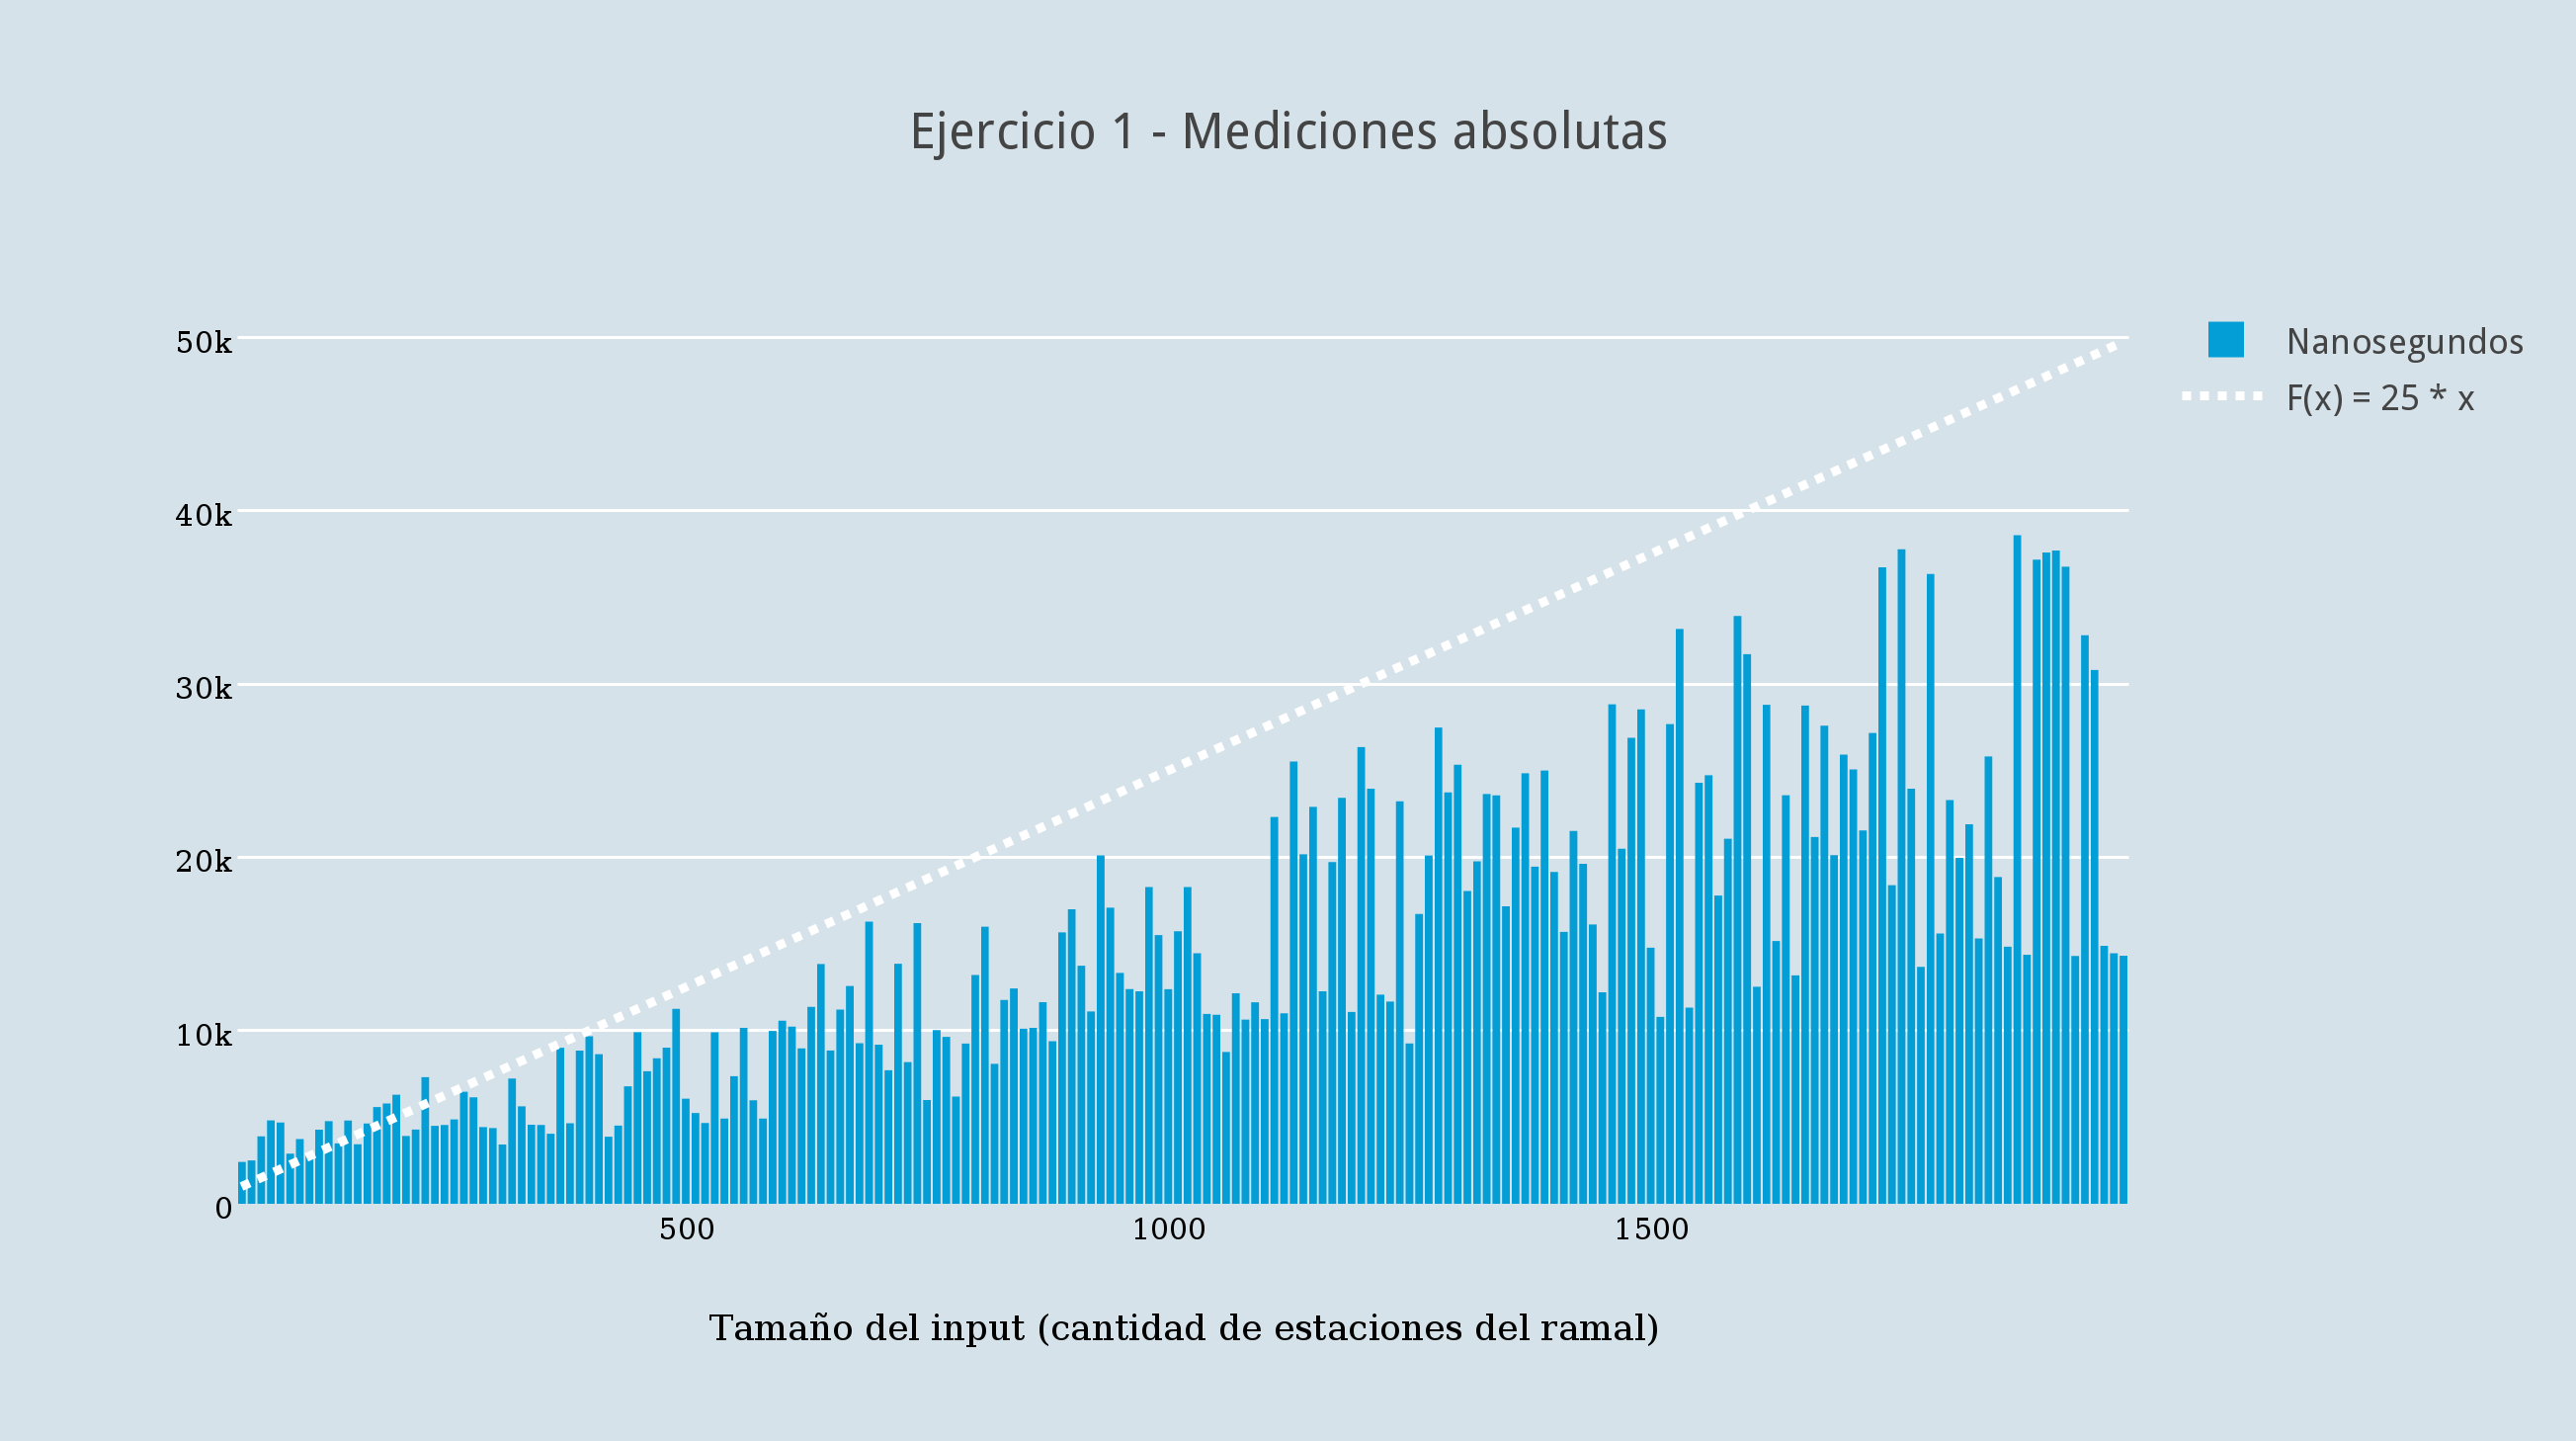
\includegraphics[scale=0.8]{imagenes/ej1/absolutas.png}
	\caption{Mediciones absolutas sobre el tamaño del input}
	\label{estacionesAbs}
   \end{center}
 \end{figure}
 
 En la figura \ref{estacionesAbs} graficamos además - a modo de referencia - la función F(x) = 25*x, con el fin de dejar en evidencia la cota superior lineal que de forma teórica dedujimos para el algoritmo que se analiza en esta sección. \\

Es conveniente aclarar que, si bien se puede vislumbrar que existe una correlación directa entre el tamaño del parámetro de entrada y los tiempos asociados a los peores casos, la gráfica presentada no es en sí la base que nos hace afirmar que la complejidad asintótica del algoritmo es lineal, si no que esta aseveración se apoya fuertemente en el estudio formal del algoritmo, esbozado en la sección \textit{An\'alisis de la complejidad}. Es decir que consideramos a los resultados obtenidos tan sólo como un sustento empírico más en favor de nuestros supuestos. En cambio, si los mismos hubieran sido inconsistentes con el análisis teórico entonces hubiesen resultado de gran relevancia a la hora de poner en tela de  juicio nuestras hipótesis iniciales. \\

 
  \begin{figure}[h!]
   \begin{center}
 	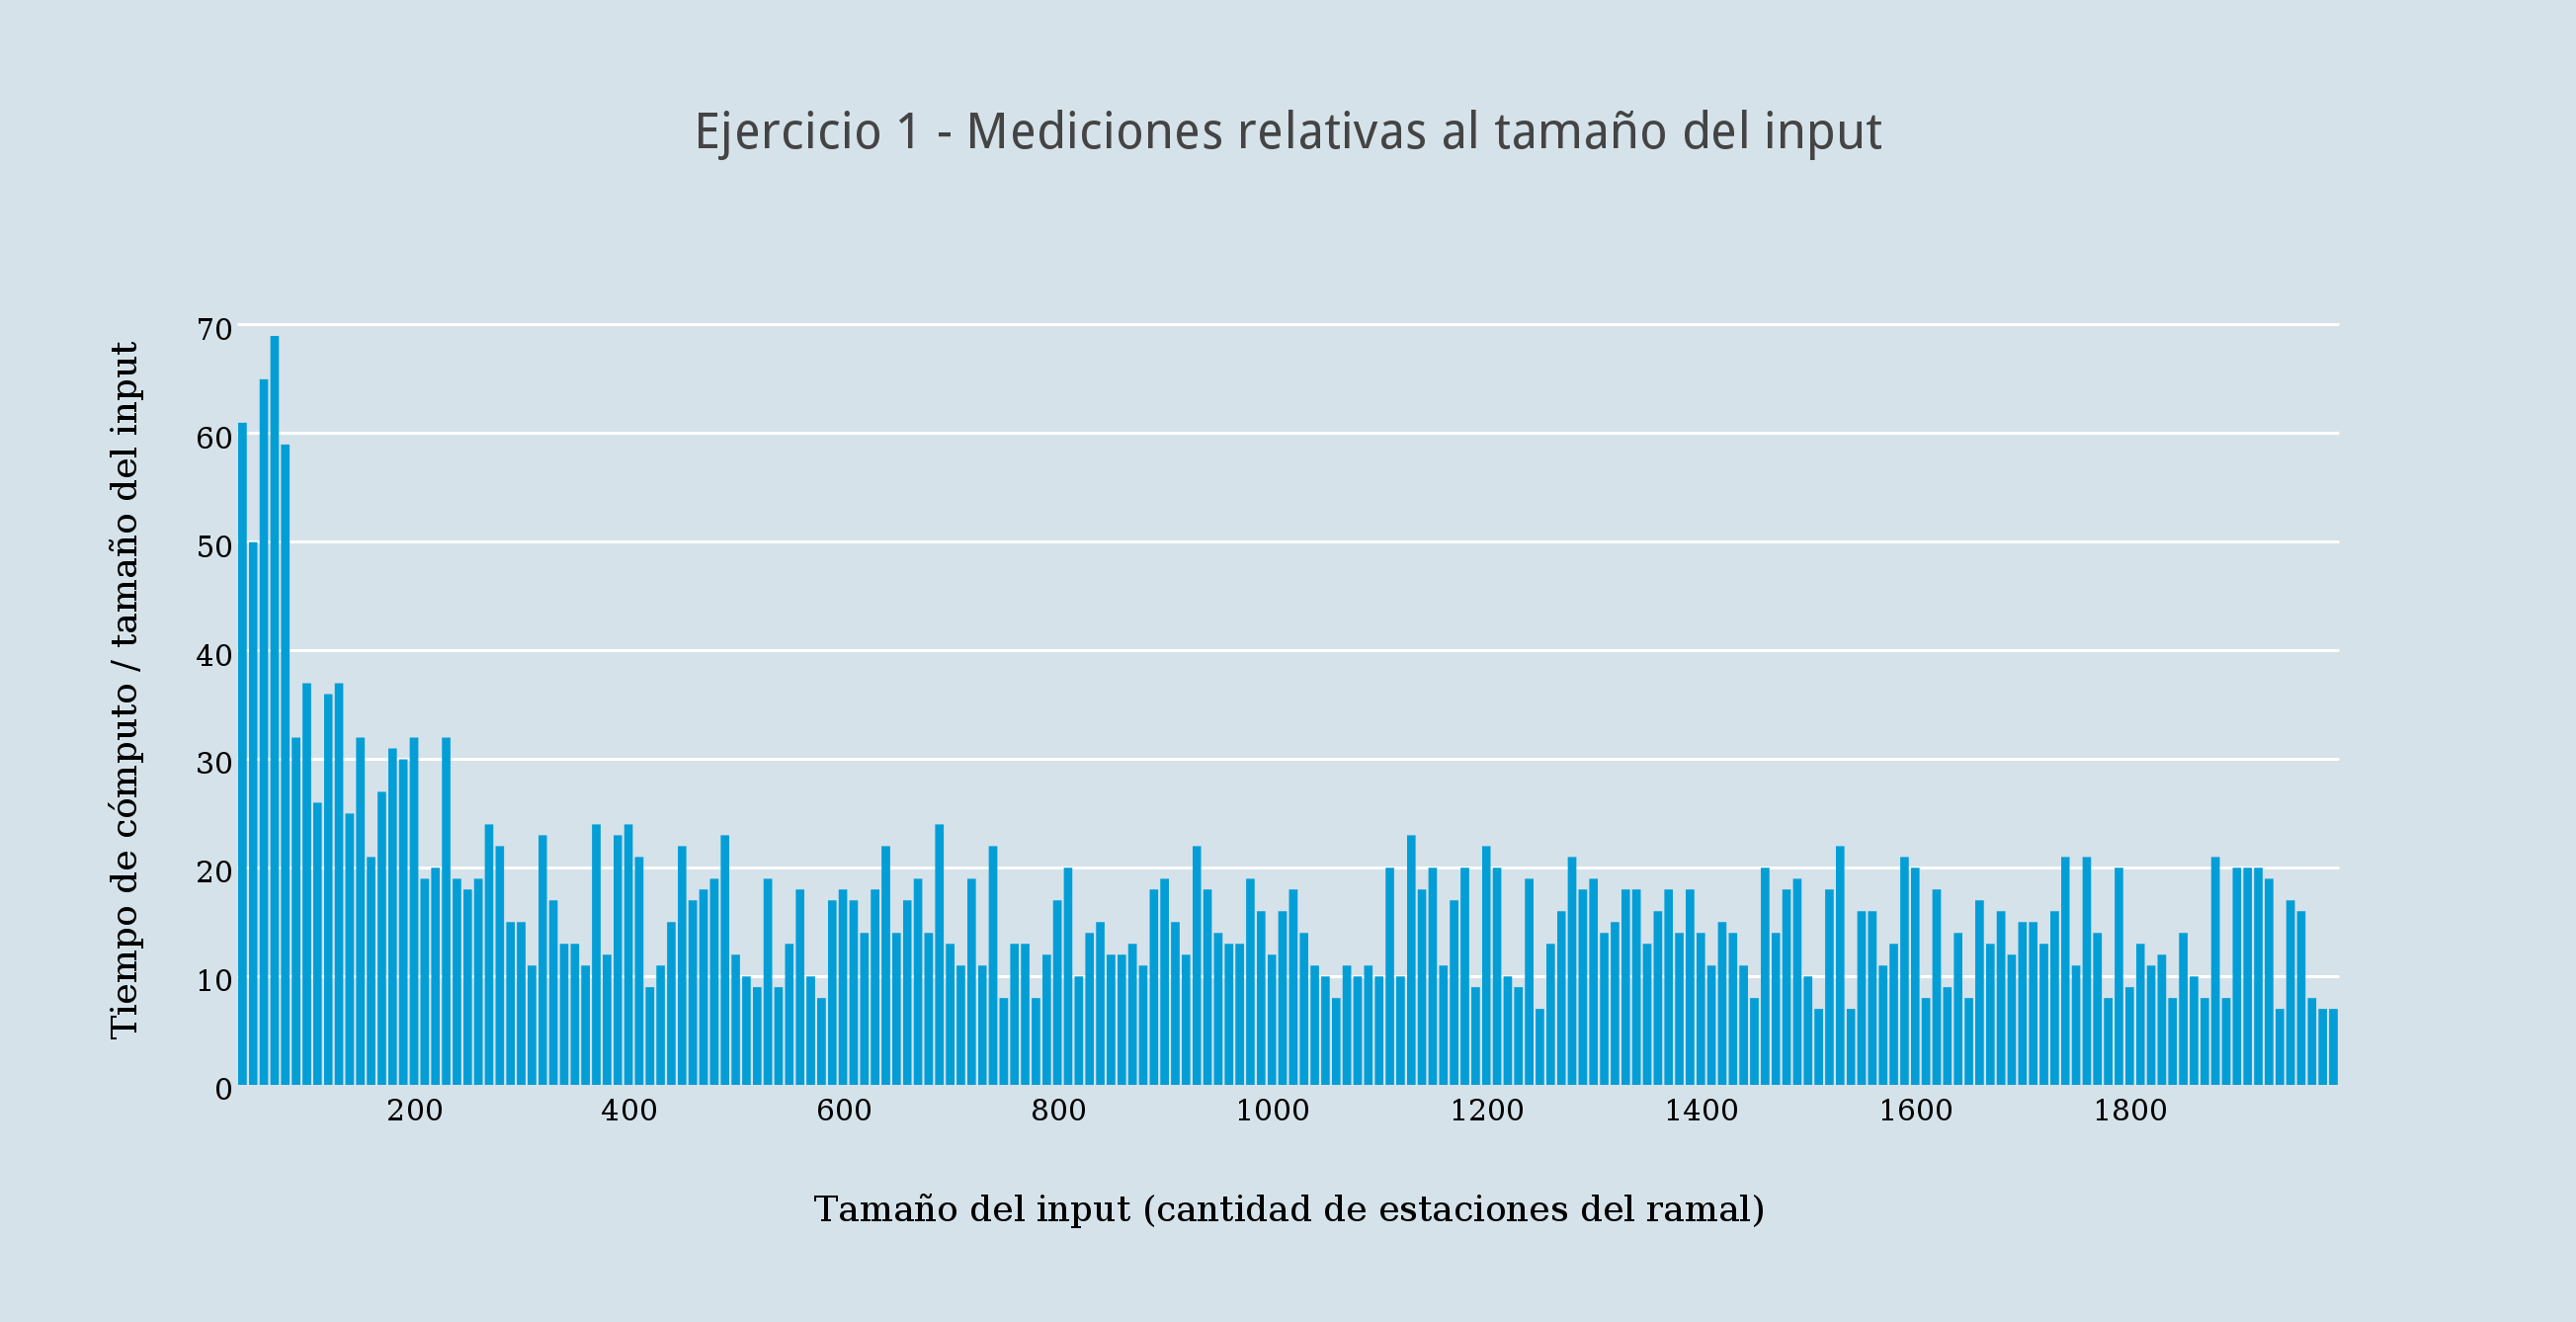
\includegraphics[scale=0.8]{imagenes/ej1/relativas.png}
	\caption{Mediciones relativas al tamaño del input}
	\label{estacionesRel}
   \end{center}
 \end{figure}

 Ahora bien, no todas las instancias aumentan su tiempo de cómputo a medida que el tamaño de la entrada se acrecienta. Esto puede deberse a varios factores, de entre los cuales consideramos necesario mencionar al menos dos:
 \begin{enumerate}[1.]
 \item {Diferencia entre instancias de casos}
 \item{Cuestiones de implementación y entorno de testing}
\end{enumerate}

En relación a las cuestiones de implementación y entorno de testing aparecen involucrados una enorme cantidad de factores que influyen al momento de realizar las pruebas, como ser:
\begin {itemize}
\item prestaciones de hardware
\item ejecución de programas y servicios del sistema operativo, de manera de manera sincrónica y paralera a la toma de mediciones
\item manejo de la memoria caché
\item ejecución del Garbaje Collector \footnote{El Garbage Collector es un proceso de baja prioridad que se ejecuta en la JVM y es el encargado de liberar la memoria que no se emplea (elimina del heap los objetos que no posean una referencia apuntándolos en el Stack). El hecho de que sea de baja prioridad implica que no puede ejecutarse en cualquier momento, si no que su comienzo se verá supeditado al manejo que haga el procesador con los trabajos de mayor prioridad. }, etc.
\end{itemize}

Si bien varios de ellos escapan a nuestro control, decidimos seleccionar las mediciones con diversos criterios previamente mencionados, de manera que los resultados fueran tan representativos como fuese posible.\\

En cuanto a los casos de prueba de performance, hemos de recordar que fueron generados de manera pseudo-aleatoria, siendo el tamaño del input el único parámetro ofrecido para la generación de las diversas instancias.\\

Es por esto que podemos ver casos donde el tamaño del input es similar y los tiempos medidos son aparentemente contradictorios.\\
Tomemos, por ejemplo, los casos de 1960 y 1970 estaciones. Si se los compara, se puede ver que para la primera instancia I$_{1}$ el valor de Tiempo( I$_{1}$) / CantEstaciones(I$_{1}$) resultó ser exactamente el doble que el obtenido mediante el cálculo de Tiempo( I$_{2}$) / CantEstaciones(I$_{2}$).\\
Observando este y otros casos llamativos, se puede comprender lo planteado observando de qué manera particular fueron instanciados los problemas \footnote{Todos los casos sobre los que fueron corridos las pruebas junto con las mediciones de tiempos correspondientes se encuentran en la carpeta /bin junto a otros datos útiles}.\\
De esta manera y haciendo un seguimiento de la implementación para estos contextos, es posible atribuir diferencias temporales tan significativas entre parámetros cuantitativamente cercanos pero cualitativamente disímiles a la longitud del cable obtenida. \\
Esto cobra sentido al observar que en el caso de menor cantidad de estaciones la longitud con la que se contaba era de aproximadamente la mitad del kilometraje que separaba a la primera ciudad de la última, mientras que en el problema resuelto para mayor cantidad de estaciones el cable llegaba a unir 1866 de 1970 estaciones desde la primera iteración principal (es decir, comparando cuántas podían unirse desde la ciudad ubicada en el Km 0).\\

Esto es consistente con lo que se puede observar si se busca que instancia tuvo la mínima razón Tiempo/TamañoInput. En nuestras pruebas ocurrió para un ramal generado de manera que la longitud del cable era tal que permitía unir 1227 de 1250 estaciones partiendo de la inicial. \footnote{Ver instancia con 1250 estaciones}\\

Todo esto tiene sentido si se observa a la luz del código, donde una simple guarda impidió que el ciclo se ejecutara una cantidad de veces mayor a la necesaria: Las líneas a las que nos referimos son 
\begin{verbatim}
 while(ramal.HayCiudadesMasLejanas() && !ramal.EsLaUltimaCiudad(indiceCiudadMasLejanaAlcanzada)) 
\end{verbatim}

Gracias a la segunda condición, podemos asegurar que el ciclo deja de ejecutarse cuando habiéndonos parado en una determinada ciudad inicial logramos alcanzar la última de las estaciones, lo cual sucede con mayor velocidad cuando no se ha de cambiar varias veces el índice de la ciudad inicial, situación que se cumple cuando el cable provisto es lo suficientemente extenso como para cubrir una cantidad considerable \footnote{Proporcional a la cantidad total de estaciones} de estaciones consecutivas.




\newpage

\newpage
\section{Problema 2: A medias}

\subsection{Descripci\'on de la problem\'atica}

\subsection{Resoluci\'on propuesta y justificaci\'on}

\subsection{An\'alisis de la complejidad}

\subsection{C\'odigo fuente}

\subsection{Experimentaci\'on}

\subsubsection{Constrastaci\'on Emp\'irica de la complejidad}


\newpage
\section{Problema 3: Girls Scouts}
\subsection{Descripción de la problemática}

En este ejercicio existe un grupo de niñas exploradoras, algunas de ellas amigas entre sí, que deben formarse en una ronda. Siendo $e$ la cantidad de exploradoras, existen $(e-1)!$ permutaciones posibles en las cuales pueden sentarse. Podemos medir la distancia entre dos amigas como la mínima cantidad de chicas que hay entre una y otra, más 1. Por ejemplo, si una chica está al lado de la otra, la distancia entre ellas es 1. Si tenemos una ronda de tres chicas, la distancia entre cualquier par de chicas va a ser 1.

El problema consiste en hallar la forma de ubicar a las exploradoras de forma tal que exista la menor distancia posible entre cada amistad, y logrando que la suma total de la distancia entre todos los pares de amigas sea mínima.

El formato de entrada es un archivo de texto que contiene una línea por cada grupo de exploradoras. Cada línea se compone de una sucesión de amistades separadas por \texttt{;} de la forma \texttt{amistad[;amistad]}. Cada amistad es un par \texttt{x xs} donde \texttt{x} es una letra y \texttt{xs} una cadena de letras.

Veamos un ejemplo. Tenemos un grupo de 5 chicas: A, B, C, D y E. A es amiga de B y C, y D es amiga de C. Esto se puede escribir de muchas maneras. Si escribimos a cada amistad dos veces, podemos hacerlo así:

\texttt{A BC;B A;C AD;D C;E}

Si las sentamos así:

\begin{tikzpicture}[auto, node distance=3cm, every loop/.style={},
                    thick,main node/.style={circle,draw,font=\sffamily\Large\bfseries}]

  \node[main node] (1) {A};
  \node[main node] (2) [below left of=1] {B};
  \node[main node] (3) [below right of=2] {E};
  \node[main node] (4) [below right of=1] {D};
  \node[main node] (5) [right of=1] {C};

  \path[every node/.style={font=\sffamily\small}]
    (1) edge node [left] {} (2)
        edge node[right] {} (5)
    (2) edge node [right] {} (1)
    (4) edge node [left] {} (5)
    (5) edge node {} (4);
\end{tikzpicture}

vamos a estar obteniendo una solución óptima, ya que la suma total de distancias es 3 (contando a cada amistad una sola vez) y la distancia máxima es 1.

El formato de salida para cada grupo de exploradoras es una línea de texto donde se debe indicar la distancia máxima obtenida, seguida de un espacio y una cadena de letras que indica la forma en que fueron sentadas las exploradoras. En caso de haber obtenido más de una solución, se debe devolver la primera en órden alfabético. Para el último ejemplo, la forma de codificar sería así:

\texttt{1 ACDEB}

Nótese que es equivalente a esta otra: \texttt{1 CDEBA}, ya que la única diferencia es por cuál exploradora empezamos a describir la ronda.

%El algoritmo a implementar debe hallar, utilizando backtracking, la permutación en donde la separación entre las niñas que son amigas sea mínima. La técnica algorítmica para resolver el problema puede reducirse a una decisión simple en cada paso: para cada posicion, determinar a qué niña colocar. La mecánica del backtracking busca detectar las instancias en donde los resultados serán peores que el mejor caso registrado, independientemente de las decisiones que se tomen adelante en esa misma rama; de esta forma, se evita el computo de permutaciones que no resultarán óptimas.


\subsection{Algoritmo desarrollado}

Desarrollamos un algoritmo que utiliza la técnica de \textit{backtracking}. Esta técnica consiste en generar de forma incremental candidatos parciales para formar soluciones, haciéndolo de manera tal de poder, en cada paso, evaluar si completar la solución parcial puede resultar en una solución válida o no. De esta manera, si se decide que no se pueden generar soluciones válidas a partir del candidato parcial, se puede abandonar la generación de todas las soluciones que derivan de éste.



La mecánica del algoritmo recursivo consiste en encontrar la mejor permutación posible desde determinada posición (dejando fijos los i primeros elementos).
Para esto, el algoritmo fija un valor en la posición i-esima y se llama recursivamente. Al volver de la recursion, se cambia el valor en la posición i-esima y se vuelve a llamar a la recursion, hasta que se hayan probado todos los valores posibles.
Cuando se detecta una instancia mejor a la anterior, se guarda una copia de la misma, y se recupera posteriormente si no se ha detectado un mejor caso.

\subsection{Justificación de correctitud}

\subsection{Análisis de la complejidad temporal}
La cantidad de posibles permutaciones para una ronda es de '(e-1)!'; en el peor escenario posible, los datos de entradas tienen un orden tal que el algoritmo encuentre una mejor situación en cada iteración, por lo cual tendrá que recorrer las '(e-1)!' permutaciones. 

En cada colocación de una exploradora, se deberá calcular que distancia existe entre ella y sus amigas, lo cual en un peor caso tiene un costo de O(a ln a)
Entonces, en el peor caso, la complejidad del algoritmo pertenece a $O( (e-1)! e a ln a), == O( (e)! a ln a)$,   lo cual es menor que $O(ee a lna) (e! < e^e)$, menor a  $O(ee a2) (a ln a < a^2)$

\subsection{Tests de correctitud}

\subsection{Experimentación para observar la performance real}

\subsubsection{Peor caso}

\subsubsection{Caso promedio}

\newpage





% \section{Contexto}

% \begin{figure}
%   \begin{center}
% 	
\includegraphics[scale=0.66]{imagenes/logouba.jpg}
% 	\caption{Descripcion de la figura}
% 	\label{nombreparareferenciar}
%   \end{center}
% \end{figure}


% \paragraph{\textbf{Titulo del parrafo} } Bla bla bla bla.
% Esto se muestra en la figura~\ref{nombreparareferenciar}.


% %\section{Enunciado y solucion} 
% %\input{enunciado}

% \section{Conclusiones y trabajo futuro}

\end{document}

